\chapter{Architecture}\label{chapter:architecture}

The proposed architecture consists in two steps, a training step and test step: the training step is shown in Figure \ref{figure:train-flow} and the test tep is shown in Figure \ref{figure:test-flow}. The training step consists in extract features from real Android methods and use that combined with the real classes to train classifiers. The first step to create the classifiers to is to have a list of fully implemented Android APIs and a list of already classified methods.

The APIs used in this work have been selected from two different repositories: the default repository of Android images used by \cite{rasthofer2014machine} and the second repository is a well known set of Android images, provided by \cite{hiddenapi}, which is used by mobile developers that need methods available only in fully implemented APIs, that are only available when the API is extracted from real devices. The APIs from level 3 to 17 used in this work were extracted from \cite{rasthofer2014api} and the APIs 17, 19 and 21 to 27 gathered from \cite{hiddenapi}. These two APIs repositories meet the requirement imposed by \cite{rasthofer2014machine}, and consists that the APIs used need to have the fully method implementation, done by extracting APIs from real devices.

\begin{figure}[!h]
    \begin{center}
        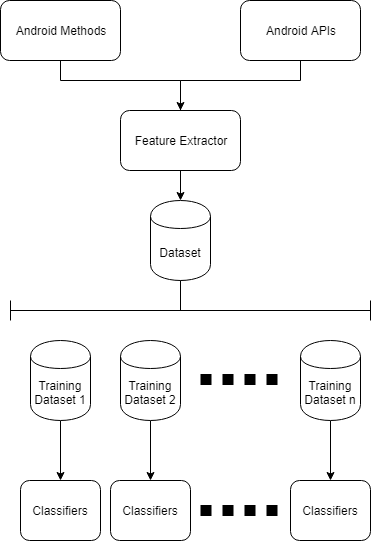
\includegraphics[width=0.5\linewidth]{images/architectures-training.png}
    \end{center}
    \caption{%
        Overview of the proposed training flow. First, the feature extractor uses Android Methods and %
        Android APIs to create a dataset, which will be sampled into other 30 different datasets that will be used %
        to train the classifiers.%
    }\label{figure:train-flow}
    \vspace{4ex}
\end{figure}

If the extraction is made using an emulator, instead of a real device, the API comes without the complete method implementation, called method stubs. As long as the taint tracker try to execute or extract runtime information from any of these methods stubs, an exception is thrown and the execution is stopped. The fully implemented methods are important due to information tracking that is done during the feature extraction, if a API method calls another method that is a source of sensitive data, the method potentially be a source of data too. Another point is that some of syntactic features are extracted from data flow inside those methods, if no method implementation were given, those features could not be computed.

In addition to the APIs, it is necessary to have a starting list of Android methods that have been hand classified, called hand annotated methods.  The feature extractor will use the hand annotated methods and the API to generate the methods features and if possible, infer the classes of non annotated methods using static taint analysis. The result of this step is the dataset used in the classification and is described in more details in Section \ref{dset_section}. With the hand annotated methods and the APIs in hand, the following step is to apply the feature extractor to each API, concatenate all the results and remove all the repeated entries, resulting in the dataset.

After the dataset creation, 30 other datasets are randomly sampled from the original, with the objective to train and evaluate the classification algorithms using a hypothesis test. Each of these datasets are subdivided into two disjoint datasets: train and test. The train dataset consists in 80\% of the original dataset and to test the model effectiveness, the test dataset have 20\% of the original samples. This is a random division done in such a way that the resultant datasets maintain the classes proportion observed in the original, if the original has 45\% of source methods, the train and test must have a proportion close to that. The datasets are created by random sample of the original one, the algorithm calculates the classes proportion and randomly selects entries to be used in train and test keeping the proportion close to the original one.

At the end of one training step, the model is evaluated with the test dataset. The whole test step is shown in Figure \ref{figure:test-flow}, for each dataset, there is a classifier to categorize the samples. This will result in a list of samples and classified labels that are going to be compared with the original label. This generates the evaluation results, consisting in precision, recall, F1 score and accuracy, the result of each metric is saved. After the the result saved, the model is overwritten and a fresh one is used to be used back in the training step. This ensures that no information is being  transferred to the next step, forgetting all the information previously learned. And at the end of 30 steps of training and test, the mean and standard deviation of each metric is calculated and reported in the results, Section \ref{result_ending}.

\begin{figure}[!h]
    \begin{center}
        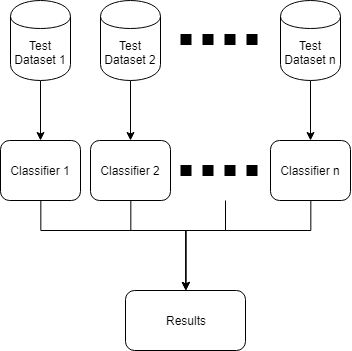
\includegraphics[width=0.5\linewidth]{images/architectures-test.png}
    \end{center}
    \caption{%
        Overview of the proposed testing flow. After the creation of datasets, the result of each classifier is used in evaluation.%
    }\label{figure:test-flow}
    \vspace{4ex}
\end{figure}
